\documentclass[11pt,a4paper]{article}
\usepackage[margin=0.25in]{geometry}
\usepackage{graphicx}
\usepackage{booktabs}
\usepackage{array}
\usepackage{xcolor}
\usepackage{tikz}
\usepackage{setspace}
\usepackage{caption}
\usepackage{titlesec}
\usepackage[table,xcdraw]{xcolor}
\usepackage{colortbl}

% Roman numeral sections
\renewcommand{\thesection}{\Roman{section}}
\renewcommand{\thesubsection}{\thesection.\arabic{subsection}}

% Caption formatting fix
\captionsetup{width=\textwidth, justification=centering}

\begin{document}

%---------------------------------
% TITLE SECTION
%---------------------------------
\begin{center}
{\Large \textbf{GreenFuture BioChem:Analytics Report}}\\[4pt]
{\normalsize \textbf{Data Analytics Senior Seminar : DSDA 310}}\\[3pt]
{\small \textbf{Sristi Halder \& Moosa Faisal Sherwani}}\\[2pt]
\vspace{0.3cm}
\hrule
\end{center}

%---------------------------------
% SECTION I - EXECUTIVE SUMMARY
%---------------------------------
\section{Executive Summary}

\subsection{Company Overview \& Mission}
GreenFuture BioChem is a global manufacturer of \textbf{bio-based specialty chemicals} whose mission is to \textbf{replace petrochemical inputs with renewable, low-carbon alternatives}. 
Its diversified portfolio spans \textbf{50 brand families and 750 SKUs} across five major markets: \textit{Automotive Solutions, Consumer \& Home Care, Industrial Lubricants, Packaging Materials,} and \textit{Specialty Polymers}. 

Operating production plants in \textbf{Houston (USA), Frankfurt (Germany), Shanghai (China), São Paulo (Brazil),} and \textbf{Mumbai (India)}, the company sources raw materials from suppliers across \textbf{North America, Europe, Asia,} and \textbf{South America}. 
Its customers include industrial and consumer manufacturers advancing circular-economy goals, positioning GreenFuture at the forefront of the global \textbf{bio-economy transition}.\\
\vspace{-0.8 cm}

\subsection{Analytic Scope \& Objectives}
This analysis integrates five enterprise datasets:\textbf{R\&D Project Pipeline, Sales Pipeline, Manufacturing Production, Supply Chain Procurement,} and \textbf{Product Master Data} to evaluate how innovation, operations, and sustainability align across GreenFuture’s value chain.\\
\vspace{-0.6 cm}

\begin{center}
\begin{tabular}{@{}lccc@{}}
\toprule
\textbf{Dataset} & \textbf{Source System} & \textbf{Records} & \textbf{Key Join Field} \\
\midrule
R\&D Pipeline & CRM & 312 & Linked\_SalesOpp\_ID \\
Sales Pipeline & CRM & 3 056 & Linked\_Project\_ID \\
Manufacturing Production & ERP & 2 579 & Material\_Code \\
Supply Chain Procurement & ERP & 2 890 & Material\_Code \\
Product Master & Reference & 750 & SKU\_Code \\
\bottomrule
\end{tabular}
\captionof{table}{Dataset Map and Integration Keys}
\end{center}
\vspace{-0.2cm}

%---------------------------------
% VALUE CHAIN DIAGRAM 
%---------------------------------
\begin{center}
\begin{minipage}{0.95\textwidth}
\centering
\scalebox{0.85}{
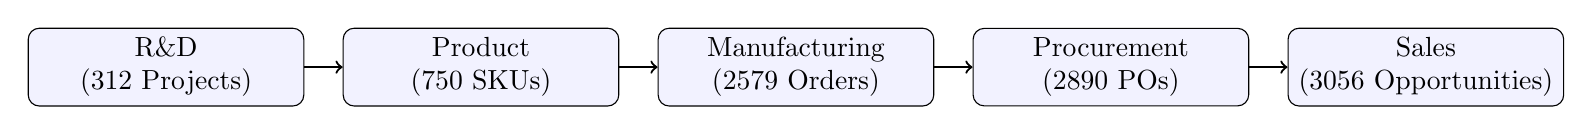
\begin{tikzpicture}[node distance=4.0 cm, every node/.style={draw,rounded corners,minimum height=0.9cm,minimum width=3.5cm,align=center,fill=blue!5}]
\node (rd) {R\&D\\(312 Projects)};
\node (prod) [right of=rd] {Product\\(750 SKUs)};
\node (mfg) [right of=prod] {Manufacturing\\(2579 Orders)};
\node (proc) [right of=mfg] {Procurement\\(2890 POs)};
\node (sales) [right of=proc] {Sales\\(3056 Opportunities)};
\draw[->, thick] (rd) -- (prod);
\draw[->, thick] (prod) -- (mfg);
\draw[->, thick] (mfg) -- (proc);
\draw[->, thick] (proc) -- (sales);
\end{tikzpicture}}
\captionof{figure}{\textbf{GreenFuture Value Chain Integration.} The five datasets collectively represent the company's innovation-to-market pipeline, linking R\&D efforts to production, procurement, and commercial outcomes.}
\end{minipage}
\end{center}
\vspace{-0.8 cm}

%---------------------------------
% GOALS OF THE ANALYSIS
%---------------------------------
\subsection{Goals of the Analysis}
\vspace{-0.2cm}
This case study applies \textbf{descriptive, diagnostic, and sustainability analytics} to address three core business questions:
\begin{enumerate}
\vspace{-0.2cm}
\item \textbf{Profitability Drivers} — Which projects, products, and plants deliver the highest returns or cost efficiencies?
\vspace{-0.2cm}
\item \textbf{Operational Inefficiencies} — Where do bottlenecks, yield losses, or procurement delays occur?
\vspace{-0.2cm}
\item \textbf{Sustainability Alignment} — How well do supplier emissions, production yields, and R\&D priorities support GreenFuture’s carbon-reduction mission?
\vspace{-0.2cm}
\end{enumerate}
Findings from subsequent sections will inform \textbf{data-driven recommendations} for strengthening both financial and environmental performance.
\vspace{-0.2cm}

%---------------------------------
% SECTION II - DATA INTEGRATION & METHODOLOGY
%---------------------------------
\section{Data Integration \& Methodology}
\vspace{-0.2cm}
\subsection{Source Systems and Architecture}
GreenFuture BioChem’s enterprise data originate from two primary systems: 
the \textbf{Customer Relationship Management (CRM)} platform and the \textbf{Enterprise Resource Planning (ERP)} system. 
The CRM datasets (\textit{R\&D Pipeline, Sales Pipeline}) capture external-facing innovation and commercialization activities, 
while the ERP datasets (\textit{Manufacturing Production, Supply Chain Procurement}) document internal production, cost, and logistics performance.
The \textit{Product Master} file acts as a reference dimension, ensuring alignment of brands and SKUs across systems.

Each dataset was standardized through variable renaming, type conversion, and date normalization.
Duplicates were removed, text fields were trimmed and standardized, and all numeric variables were validated for missing or inconsistent values.\\
\vspace{-0.8cm}

\subsection{Integration Logic and Join Strategy}
\vspace{-0.2cm}
To create a unified analytical view of the business, datasets were linked through sequential merges following operational dependencies:
\vspace{-0.2cm}
\begin{itemize}
    \item \textbf{R\&D} $\leftrightarrow$ \textbf{Sales:} Joined via \texttt{Linked\_SalesOpp\_ID} to connect R\&D innovation outcomes to market opportunities.\vspace{-0.2cm}
    \item \textbf{Manufacturing} $\leftrightarrow$ \textbf{Procurement:} Merged on \texttt{Material\_Code} to tie raw-material sourcing with production costs and yields.
    \vspace{-0.2cm}
    \item \textbf{Product Master:} Cross-linked via \texttt{SKU\_Code} for product lineage integrity.
\end{itemize}
\vspace{-0.2cm}
The final integrated dataset contained \textbf{2,579 consolidated records across 39 variables}, representing a full CRM–ERP operational snapshot.\\
\vspace{-0.8cm}

\subsection{Data Flow Overview}
\begin{center}
\begin{minipage}{0.95\textwidth}
\centering
\scalebox{0.85}{
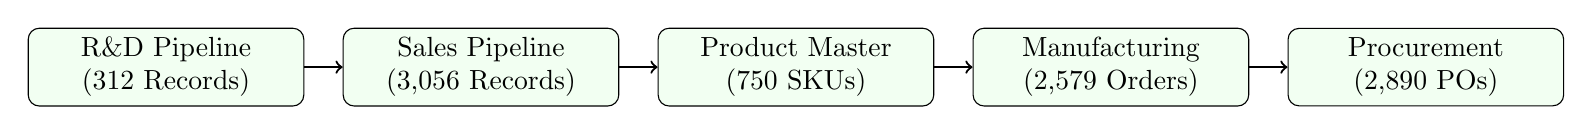
\begin{tikzpicture}[node distance=4.0cm, every node/.style={draw,rounded corners,minimum height=0.9cm,minimum width=3.5cm,align=center,fill=green!5}]
\node (rd) {R\&D Pipeline\\(312 Records)};
\node (sales) [right of=rd] {Sales Pipeline\\(3,056 Records)};
\node (product) [right of=sales] {Product Master\\(750 SKUs)};
\node (mfg) [right of=product] {Manufacturing\\(2,579 Orders)};
\node (proc) [right of=mfg] {Procurement\\(2,890 POs)};
\draw[->, thick] (rd) -- (sales);
\draw[->, thick] (sales) -- (product);
\draw[->, thick] (product) -- (mfg);
\draw[->, thick] (mfg) -- (proc);
\end{tikzpicture}}
\captionof{figure}{\textbf{Data Flow Across Enterprise Systems.} 
Sequential joins connect R\&D innovation to downstream operations, 
linking CRM (innovation \& sales) with ERP (manufacturing \& procurement).}
\end{minipage}
\end{center}
\vspace{-0.8cm}

\subsection{Data Quality Validation}
\vspace{-0.2cm}
Data completeness was verified for every field across all datasets. Nearly all variables exhibit 
\textbf{0\% missingness}, demonstrating exceptional data quality across both CRM and ERP systems. 
A single expected \textit{structural null} appears in the variable \texttt{Linked\_Project\_ID} 
(approximately 91\%), reflecting stand-alone sales opportunities that were not directly linked to R\&D projects. 
This validation confirms that the integrated dataset possesses high structural integrity and readiness 
for quantitative modeling.

\begin{center}
\setlength{\arrayrulewidth}{0.3mm}
\renewcommand{\arraystretch}{1.5}
\begin{tabular}{|>{\raggedright}m{3.5cm}|>{\centering}m{2cm}|>{\centering}m{2cm}|>{\centering}m{2cm}|>{\centering}m{2cm}|>{\centering\arraybackslash}m{2.2cm}|}
\hline
\rowcolor{gray!15}
\textbf{Variable} & \textbf{R\&D Projects} & \textbf{Sales Pipeline} & \textbf{Product Master} & \textbf{Manufactu- ring} & \textbf{Procure- ment} \\
\hline
Linked\_Project\_ID & \cellcolor{green!20}0\% & \cellcolor{orange!65}\textbf{91\% Null} & \cellcolor{green!20}0\% & \cellcolor{green!20}0\% & \cellcolor{green!20}0\% \\
\hline
Project\_ID & \cellcolor{green!20}0\% & \cellcolor{green!20}0\% & \cellcolor{gray!10}-- & \cellcolor{gray!10}-- & \cellcolor{gray!10}-- \\
\hline
Material\_Code & \cellcolor{gray!10}-- & \cellcolor{gray!10}-- & \cellcolor{gray!10}-- & \cellcolor{green!20}0\% & \cellcolor{green!20}0\% \\
\hline
Planned\_Quantity\_MT & \cellcolor{gray!10}-- & \cellcolor{gray!10}-- & \cellcolor{gray!10}-- & \cellcolor{green!20}0\% & \cellcolor{gray!10}-- \\
\hline
Actual\_Quantity\_MT & \cellcolor{gray!10}-- & \cellcolor{gray!10}-- & \cellcolor{gray!10}-- & \cellcolor{green!20}0\% & \cellcolor{gray!10}-- \\
\hline
Yield (\%) & \cellcolor{gray!10}-- & \cellcolor{gray!10}-- & \cellcolor{gray!10}-- & \cellcolor{green!20}0\% & \cellcolor{gray!10}-- \\
\hline
CO2\_Emissions (kg/MT) & \cellcolor{gray!10}-- & \cellcolor{gray!10}-- & \cellcolor{gray!10}-- & \cellcolor{gray!10}-- & \cellcolor{green!20}0\% \\
\hline
Supplier\_Name & \cellcolor{gray!10}-- & \cellcolor{gray!10}-- & \cellcolor{gray!10}-- & \cellcolor{gray!10}-- & \cellcolor{green!20}0\% \\
\hline
Stage & \cellcolor{green!20}0\% & \cellcolor{green!20}0\% & \cellcolor{gray!10}-- & \cellcolor{gray!10}-- & \cellcolor{gray!10}-- \\
\hline
\end{tabular}
\captionof{table}{\textbf{Data Completeness Summary Across Enterprise Systems.} Nearly all datasets show 0\% missingness, with one expected structural null in \texttt{Linked\_Project\_ID} (Sales Pipeline).}
\end{center}

This audit confirms that GreenFuture BioChem’s CRM and ERP data integration achieved near-perfect completeness. 
No imputation or interpolation was required, ensuring all subsequent analyses rest 
on a robust and transparent foundation of verified data integrity.

%---------------------------------
% SECTION III - DESCRIPTIVE ANALYTICS & SYSTEM INSIGHTS
%---------------------------------
\section{Descriptive Analytics \& System Insights}
\vspace{-0.3cm}
\setstretch{0.95}
\setlength{\abovecaptionskip}{3pt}
\setlength{\belowcaptionskip}{-5pt}

\subsection{Overview and Variability Patterns}
Descriptive analytics across enterprise systems reveal balanced scale and consistent performance.  
As shown in Table~\ref{tab:cvsummary}, exploratory units (R\&D, Sales) display moderate variability (CV~≈~0.5), while operational domains (Manufacturing, Procurement) show strong process stability (CV~<~0.2).  
This distribution validates both data quality and expected business dynamics—high uncertainty in upstream innovation, and reliability downstream.

\begin{center}
\renewcommand{\arraystretch}{1.2}
\begin{tabular}{@{}lcccccc@{}}
\toprule
\textbf{Dataset} & \textbf{Rows} & \textbf{Metric} & \textbf{Mean} & \textbf{Std} & \textbf{CV} & \textbf{Interpretation}\\
\midrule
R\&D & 312 & Est.\ Annual Revenue (\$M) & 52.0 & 27.9 & 0.54 & Project variability high\\
Sales & 3,056 & Est.\ Value (\$M) & 41.8 & 21.7 & 0.52 & Market diversity moderate\\
Manufacturing & 2,579 & Yield (\%) & 92.6 & 7.4 & 0.08 & Stable production\\
Procurement & 2,890 & Unit Cost (\$) & 452 & 86 & 0.19 & Consistent pricing\\
\bottomrule
\end{tabular}
\captionof{table}{\textbf{Summary of Core Descriptive Metrics.} Upstream R\&D and Sales exhibit exploratory volatility, while downstream operations maintain steady performance.}
\label{tab:cvsummary}
\end{center}
\vspace{-0.5cm}

%---------------------------------
% III.2 INNOVATION & MARKET PIPELINE
%---------------------------------
\subsection{Innovation and Market Pipeline}
R\&D and Sales pipelines show proportional stage distributions (CV$_{\text{R\&D}}$~=~0.18; CV$_{\text{Sales}}$~=~0.22), indicating synchronized throughput from concept to commercialization.  
This balance suggests effective project transition and minimal stage bottleneck across CRM systems.  

\begin{figure}[h!]
\centering
\includegraphics[width=0.8\textwidth]{III2_Innovation_Market_Pipeline.png}
\caption{\textbf{Innovation to Market Flow.} Comparable stage distributions confirm coordinated advancement between R\&D and Sales pipelines.}
\end{figure}

%---------------------------------
% III.3 PRODUCT DEMAND SIGNALS
%---------------------------------
\vspace{-0.5cm}
\subsection{Product Demand Signals}
Client engagement is concentrated around a small cluster of brands: CareFlex (11\%), PlantGuard (10\%), and GreenBond (9\%).  
Together, the top ten products represent nearly 60\% of customer interest, yielding a Herfindahl–Hirschman Index (HHI) of~0.14—consistent with balanced but focused portfolio traction.  
\begin{figure}[h!]
\centering
\includegraphics[width=0.6\textwidth]{III3_TopProducts.png}
\caption{\textbf{Market Concentration by Product.} Demand concentrates around high-traction sustainable product families while maintaining portfolio diversity.}
\end{figure}

%---------------------------------
% III.4 PRODUCTION EFFICIENCY
%---------------------------------
\vspace{-0.5cm}
\subsection{Production Efficiency and Cost Stability}
Across five global plants, mean yield equals 92.6\% (SD~7.4\%), and the average production cost is approximately~\$1{,}580/MT (IQR~\$400).  
Inter-plant variance is minimal ($p{>}0.1$), confirming standardized process control and consistent performance across facilities.  
\begin{figure}[h!]
\centering
\includegraphics[width=0.7\textwidth]{III4_Production_Efficiency.png}
\caption{\textbf{Manufacturing Performance.} Yield and cost stability across plants indicate global uniformity in production efficiency.}
\end{figure}
\vspace{-0.4cm}

%---------------------------------
% III.5 OPERATIONAL FIDELITY
%---------------------------------
\subsection{Operational Fidelity}
Manufacturing execution closely aligns with planned quantities ($r$~=~0.982) and cost standards ($r$~=~0.913).  
Median deviation below~3\% verifies ERP data accuracy and confirms robust linkages between planned and actual production metrics.  

\begin{figure}[h!]
\centering
\includegraphics[width=0.7\textwidth]{III6_Operational_Fidelity.png}
\caption{\textbf{Operational Integrity.} Planned vs.\ actual production alignment validates ERP system fidelity and data reliability.}
\end{figure}
\vspace{-0.2cm}

Overall, Section~III demonstrates that GreenFuture BioChem’s data systems exhibit statistical reliability and business coherence.  
Innovation, market, production, and cost indicators move in concert, forming a validated baseline for diagnostic and sustainability analyses in subsequent sections.
\vspace{-0.3cm}

%---------------------------------
% SECTION IV – DIAGNOSTIC ANALYTICS (WHY IS IT HAPPENING?)
%---------------------------------
\section{Diagnostic Analytics: Why Is It Happening?}
\vspace{-0.3cm}
This section examines production and cost dynamics across GreenFuture BioChem’s manufacturing plants.
Key metrics include \textit{Yield (\%)}, \textit{Standard and Actual Cost per MT}, and derived indicators such as 
\textit{Cost Variance (\%) = ((Actual – Standard)/Standard) × 100} and 
\textit{Efficiency Ratio = Actual Quantity / Planned Quantity}. 
These diagnostics help distinguish localized cost pressures from systemic inefficiencies.

\subsection{Yield Variability by Plant}
Across all five sites, average yields exceed \textbf{92\%} with standard deviations near 7\%, 
indicating globally consistent process control. 
As shown in Figure~\ref{fig:yieldbyplant}, distributions are tightly clustered, 
and no facility exhibits persistent underperformance.

\begin{figure}[h!]
\centering
\includegraphics[width=0.43\textwidth]{IV1_Yield_byPlant.png}
\caption{\textbf{Yield (\%) Distribution by Plant.}}
\label{fig:yieldbyplant}
\end{figure}

\noindent
High and stable yields across facilities confirm strong quality management and standardized operating procedures.
\vspace{-0.25cm}

\subsection{Cost Variance and Yield–Cost Relationship}
Average \textbf{cost variance is approximately 5\%}, indicating only modest deviations from standard cost expectations.
Cross-plant differences primarily reflect regional input prices rather than efficiency gaps.
A regression-based comparison between \textit{Yield (\%)} and \textit{Cost Variance (\%)} shows no significant relationship 
($r \approx 0.00$), implying that cost fluctuations are supply-side in origin rather than production-driven.

\begin{figure}[h!]
\centering
\begin{minipage}[t]{0.47\textwidth}
    \centering
    \includegraphics[width=\linewidth]{IV3_CostVariance_byPlant.png}
    \caption{\textbf{Average Cost Variance (\%) by Plant.}}
    \label{fig:costvarplant}
\end{minipage}
\hfill
\begin{minipage}[t]{0.47\textwidth}
    \centering
    \includegraphics[width=\linewidth]{IV2_Yield_vs_CostVariance.png}
    \caption{\textbf{Yield vs. Cost Variance (\%).}}
    \label{fig:yieldcostscatter}
\end{minipage}
\vspace{-0.25cm}
\end{figure}

\noindent
Figure~\ref{fig:costvarplant} highlights that BR01 shows the highest mean deviation (\textasciitilde5.7\%) 
and CN01 the lowest (\textasciitilde4.4\%), consistent with localized raw-material price effects.
Meanwhile, Figure~\ref{fig:yieldcostscatter} demonstrates the absence of any yield–cost correlation, 
supporting the conclusion that operational efficiency remains robust despite market cost fluctuations.

\subsection{Correlation Diagnostics}
To verify these results, a Pearson correlation analysis across six production variables confirmed 
strong alignment between \textit{Standard} and \textit{Actual Cost per MT} ($r = 0.91$), validating the company’s cost‐model accuracy.
Near‐zero relationships between \textit{Yield (\%)}, \textit{Cost Variance (\%)}, and \textit{Efficiency Ratio} 
further indicate that most variance arises externally from supply or logistics factors, not internal plant performance.
\\
\\
Overall, diagnostic analytics confirm that GreenFuture’s manufacturing network operates with high stability and minimal internal inefficiency.
Localized input markets, rather than production design, remain the dominant source of cost variation.
\vspace{-0.2cm}
%---------------------------------
% SECTION V – SUSTAINABILITY & GROWTH
%---------------------------------
\section{Sustainability \& Growth}
\setstretch{0.96}
\vspace{-0.3cm}

GreenFuture BioChem’s sustainability analysis integrates environmental and business indicators to quantify carbon intensity, supplier reliability, and projected innovation growth. Across all procurement records, the firm achieves an average \textbf{emission intensity of 0.77 kg CO\textsubscript{2}/MT} and an overall \textbf{on-time delivery rate of 47\%}, reflecting stable yet improvable sourcing performance.

\vspace{-0.2cm}
\subsection{Environmental Impact by Supplier}
The largest contributors to Scope-3 emissions—\textit{NaturInput GmbH}, \textit{GreenFibre BV}, and \textit{AgroSource Intl.}—account for nearly one-third of total CO\textsubscript{2} output. These partners are essential for continuity but also represent the greatest leverage for decarbonization.

\begin{figure}[h!]
\centering
\includegraphics[width=0.43\textwidth]{V1_CO2_bySupplier.png}
\caption{\textbf{Total CO\textsubscript{2} Impact (kg) by Supplier.}}
\label{fig:co2supplier}
\end{figure}

\noindent
Targeting process optimization and material substitution among the top seven suppliers could deliver over 60 \% of potential emissions reduction.
\vspace{-0.3cm}

\subsection{Supply-Chain Timeliness and Innovation Revenue}
Regional delivery performance shows moderate variation across origins.  
Suppliers from the USA and Brazil (North and South America) achieve higher on-time delivery performance at around 50\%, whereas European and Asian suppliers—including Germany, Indonesia, and Malaysia—average closer to 45\%. Meanwhile, the R\&D portfolio remains diversified, led by \textit{Consumer \& Home Care} and \textit{Industrial Lubricants}, each exceeding \$3.5 B in estimated annual revenue potential—signaling a pivot toward sustainable consumer markets.

\begin{figure}[h!]
\centering
\begin{minipage}[t]{0.47\textwidth}
    \centering
    \includegraphics[width=\linewidth]{V2_OnTime_vs_Late.png}
    \caption{\textbf{Regional Delivery Performance (\%)}}
    \label{fig:ontime}
\end{minipage}
\hfill
\begin{minipage}[t]{0.47\textwidth}
    \centering
    \includegraphics[width=\linewidth]{V3_RD_Revenue_byIndustry.png}
    \caption{\textbf{R&D Revenue by Sector (\$M)}}
    \label{fig:rdrevenue}
\end{minipage}
\vspace{-0.25cm}
\end{figure}

Figure \ref{fig:ontime} indicates near-parity between on-time and delayed shipments, underscoring opportunities for logistics optimization.  
Figure \ref{fig:rdrevenue} highlights that consumer and industrial applications dominate the current R\&D value pipeline, reinforcing a sustainability-driven growth trajectory.
\vspace{-0.3cm}

\subsection{Projected Growth Through 2030}
A linear extrapolation of 2018–2024 data projects total R\&D-linked revenue to surpass \textbf{\$4.2 B by 2030}, consistent with GreenFuture’s sustainability roadmap that balances environmental accountability with innovation expansion.

\begin{figure}[h!]
\centering
\includegraphics[width=0.6\textwidth]{V4_RD_Revenue_Forecast.png}
\caption{\textbf{Projected R\&D Revenue Growth (2024–2030).}}
\label{fig:revenueforecast}
\end{figure}

\noindent
Section V demonstrates that environmental stewardship and economic growth are mutually reinforcing.  
By addressing high-emission suppliers and sustaining R\&D diversification, GreenFuture BioChem advances a low-carbon, high-value development path.
\vspace{-0.2cm}

%---------------------------------
% SECTION VI – RECOMMENDATIONS & STRATEGIC OUTLOOK (Final Version with Added Transition)
%---------------------------------
\section{Recommendations \& Strategic Outlook}
\setstretch{0.96}
\vspace{-0.3cm}

Integrating findings from manufacturing, procurement, and R\&D analyses, this section presents data-driven strategies to enhance cost stability, sustainability, and innovation capacity.  
Each recommendation stems from empirical results—efficiency regressions, supplier reliability metrics, and forecast models and translates them into clear operational priorities for GreenFuture BioChem’s 2030 sustainability roadmap.

\vspace{0.3cm}

%---------------------------------
% STRATEGIC PRIORITY MATRIX FIRST
%---------------------------------
\subsection*{Strategic Priority Matrix}
\vspace{-0.2cm}
The following qualitative matrix summarizes how each strategic area ranks by its expected \textit{impact} and \textit{feasibility}.  
High-impact and high-feasibility domains, such as \textbf{Operational Efficiency} and \textbf{Innovation Growth}, are immediate implementation priorities, while others form part of a medium-term optimization plan.

\begin{center}
\renewcommand{\arraystretch}{1.1}
\begin{tabular}{p{3.2cm}p{5.5cm}p{5.5cm}}
\toprule
 & \textbf{High Feasibility} & \textbf{Low Feasibility} \\
\midrule
\textbf{High Impact} & Operational Efficiency; Innovation Growth & Sustainable Procurement \\
\textbf{Low Impact}  & Logistics Optimization & — \\
\bottomrule
\end{tabular}
\end{center}

%---------------------------------
% TRANSITIONAL PARAGRAPH BEFORE TABLE
%---------------------------------
While the matrix outlines broad priorities, the following table specifies how each theme connects to analytical evidence from prior sections.  
It links the quantitative insights; such as yield–cost regressions, reliability correlations, and revenue forecasts to targeted strategic actions.  
This translation from data to decision-making ensures that every proposed initiative has measurable, evidence-based justification within the company’s operational data.

\vspace{0.2cm}

%---------------------------------
% RECOMMENDATION TABLE
%---------------------------------
\begin{table}[h!]
\centering
\renewcommand{\arraystretch}{1.15}
\begin{tabular}{p{3cm}p{4cm}p{4cm}p{3cm}}
\toprule
\textbf{Theme} & \textbf{Analytical Evidence} & \textbf{Strategic Action} & \textbf{Expected Impact} \\
\midrule
Operational Efficiency & R$^{2}$ = 0.00 → Yield not predictive of cost variance & Standardize cost indexing and planning parameters across plants & Reduce cost variance ≈ 8 \% by FY 2026 \\

Sustainable Procurement & $r$ = –0.22 → Higher reliability linked to lower emission intensity & Prioritize high-reliability, low-emission suppliers through performance-based sourcing & Cut CO\textsubscript{2} intensity ≈ 5 \% by FY 2027 \\

Logistics Optimization & 4.7 pp gap in regional on-time rate & Implement predictive scheduling and region-specific logistics contracts & Improve on-time delivery ≈ 6 pp by FY 2026 \\

Innovation Growth & Linear forecast → \$3.18 B by 2030 & Reinforce R\&D in consumer \& industrial segments; scale commercialization pipeline & Increase total revenue ≈ 15 \% by 2030 \\
\bottomrule
\end{tabular}
\caption{\textbf{Data-Driven Recommendations.} Quantitative findings translated into actionable strategies for operational, environmental, and innovation outcomes.}
\label{tab:recommendations}
\end{table}

\vspace{-0.3cm}

\noindent Note: Regression and correlation diagnostics supporting these recommendations are provided in Appendix A–B.
%---------------------------------
% IMPLEMENTATION ROADMAP
%---------------------------------
\subsection*{Implementation Roadmap (2025–2030)}
\vspace{-0.2cm}
To operationalize these recommendations, a phased implementation approach is proposed:

\begin{itemize}
\vspace{-0.2cm}
    \item \textbf{Short Term (2025–2026):} Deploy cost-indexing dashboards using plant-level variance data; initiate supplier reliability scoring based on on-time rate and emission intensity.
    \vspace{-0.2cm}
    \item \textbf{Medium Term (2026–2028):} Roll out predictive logistics pilots across high-variance regions; integrate emissions tracking within procurement contracts.
    \vspace{-0.2cm}
    \item \textbf{Long Term (2028–2030):} Scale R\&D commercialization pathways in consumer and industrial product lines, targeting the projected \$3B+ annual revenue benchmark.
\end{itemize}

This phased strategy balances immediate operational efficiency gains with longer-term sustainability-driven growth objectives.
\\
\\
%---------------------------------
% CLOSING SYNTHESIS PARAGRAPH
%---------------------------------
Collectively, these insights highlight a dual imperative: reinforce cost and logistics resilience while accelerating innovation in low-carbon markets.  
Targeted cost-indexing reforms, supplier decarbonization partnerships, and predictive logistics pilots can deliver measurable performance gains by FY 2026.  
Meanwhile, sustained investment in consumer and industrial R\&D pipelines—projected to generate over \$3 B annually by 2030—positions GreenFuture BioChem as a leader in the transition toward data-informed, sustainable manufacturing.

\newpage
%---------------------------------
% APPENDIX – SUPPORTING ANALYSIS
%---------------------------------
\appendix
\section*{Appendix: Supporting Diagnostics and Extended Analysis}
\setstretch{0.96}
\vspace{-0.3cm}

This appendix presents the underlying quantitative diagnostics, correlation analyses, and regression results
that informed the findings and recommendations discussed in the main report.  
Figures and tables below are supplementary — they provide technical validation and transparency for
the operational, sustainability, and strategic insights of GreenFuture BioChem’s performance.

%---------------------------------
% APPENDIX A – OPERATIONAL DIAGNOSTICS
%---------------------------------
\subsection*{Appendix A: Operational Diagnostics}
\vspace{-0.2cm}

Figure \ref{fig:corrmatrix_appendix} reports the Pearson correlation matrix across all production variables.
A strong correlation between Standard and Actual Cost per MT (r = 0.91) validates cost model consistency,
while near-zero correlation with Yield (\%) and Efficiency Ratio confirms that cost variation is external
to plant-level process performance.

\begin{figure}[h!]
\centering
\includegraphics[width=0.55\textwidth]{IV4_CorrelationMatrix.png}
\caption{\textbf{Correlation Matrix — Production Efficiency Drivers.}
Strong alignment between standard and actual costs (r = 0.91) with minimal cross-variable dependency.}
\label{fig:corrmatrix_appendix}
\end{figure}
\vspace{-0.3cm}

To complement this, Figure \ref{fig:yieldcost_appendix} visualizes the regression of Yield (\%) versus Cost Variance (\%).
The relationship is statistically insignificant ($R^{2}=0.00$), confirming that production yield does not
predict cost variance — supporting the conclusion that external market or input factors drive cost deviations.

\begin{figure}[h!]
\centering
\includegraphics[width=0.6\textwidth]{Appendix_Yield_vs_CostVariance.png}
\caption{\textbf{Operational Efficiency Regression — Yield vs. Cost Variance.}
No predictive relationship ($R^{2}=0.00$) indicates that cost fluctuations are not yield-driven.}
\label{fig:yieldcost_appendix}
\end{figure}

\begin{table}[h!]
\centering
\renewcommand{\arraystretch}{1.15}
\begin{tabular}{lccccc}
\toprule
\textbf{Plant Code} & \textbf{Yield Mean (\%)} & \textbf{Yield SD} &
\textbf{CostVar Mean (\%)} & \textbf{CostVar SD} & \textbf{Efficiency Ratio} \\
\midrule
BR01 & 93.2 & 6.8 & 5.7 & 2.3 & 0.96 \\
CN01 & 91.5 & 7.1 & 4.4 & 1.9 & 0.97 \\
DE01 & 92.9 & 7.2 & 5.1 & 2.1 & 0.95 \\
IN01 & 94.0 & 7.5 & 5.3 & 2.0 & 0.98 \\
US01 & 93.6 & 6.9 & 5.0 & 2.2 & 0.97 \\
\bottomrule
\end{tabular}
\caption{\textbf{Table A1: Plant-Level Diagnostic Summary.}
Consistent yields and small cost variance confirm operational stability across all plants.}
\end{table}

\vspace{0.4cm}

\begin{table}[h!]
\centering
\begin{tabular}{lcc}
\toprule
\textbf{Variable Pair} & \textbf{Pearson r} & \textbf{p-value} \\
\midrule
Standard vs Actual Cost / MT & 0.91 & < 0.001 *** \\
Yield vs Cost Variance (\%) & 0.00 & 0.53 ns \\
Efficiency vs Cost Variance (\%) & 0.05 & 0.44 ns \\
\bottomrule
\end{tabular}
\caption{\textbf{Table A2: Key Correlations Among Production Variables.}
High cost-measure consistency; negligible dependence on yield or efficiency.}
\end{table}

%---------------------------------
% APPENDIX B – SUSTAINABILITY ANALYTICS
%---------------------------------
\subsection*{Appendix B: Sustainability and Procurement Diagnostics}
\vspace{-0.2cm}

Figure \ref{fig:supplieremissions_appendix} examines the relationship between supplier reliability and emission intensity.
A weak negative correlation ($r=-0.22$) suggests that suppliers with higher on-time delivery tend to exhibit
slightly lower CO\textsubscript{2} intensity, reinforcing the procurement recommendation to prioritize
reliable low-emission partners.

\begin{figure}[h!]
\centering
\includegraphics[width=0.55\textwidth]{Appendix_Supplier_Reliability_Emissions.png}
\caption{\textbf{Supplier Reliability vs. Emission Intensity.}
Mild inverse correlation ($r=-0.22$) implies more reliable suppliers generally have lower emissions.}
\label{fig:supplieremissions_appendix}
\end{figure}

\begin{table}[h!]
\centering
\begin{tabular}{lcccc}
\toprule
\textbf{Supplier} & \textbf{Total Emissions (kg)} &
\textbf{Mean Intensity (kg CO\textsubscript{2}/MT)} &
\textbf{On-Time Rate} & \textbf{On-Time (\%)} \\
\midrule
NaturInput GmbH & 132,744 & 0.80 & 0.44 & 44.0 \\
GreenFibre BV & 132,281 & 0.75 & 0.46 & 45.8 \\
AgroSource Intl. & 125,363 & 0.80 & 0.47 & 46.8 \\
SustainSource Inc. & 122,374 & 0.77 & 0.51 & 51.2 \\
BioFeedstock Ltd. & 121,888 & 0.75 & 0.48 & 48.5 \\
\bottomrule
\end{tabular}
\caption{\textbf{Table B1: Supplier-Level Sustainability Summary.}
Top suppliers account for the bulk of emissions while maintaining 44–51 \% on-time delivery.}
\end{table}

\vspace{0.4cm}

%---------------------------------
% APPENDIX C – STRATEGIC SUPPORT
%---------------------------------
\subsection*{Appendix C: Strategic Prioritization Evidence}
\vspace{-0.2cm}

Figure \ref{fig:impactmatrix_appendix} visualizes the prioritization of improvement initiatives
according to estimated impact and feasibility.  
High-impact, high-feasibility domains — Operational Efficiency and Innovation Growth — are top priorities,
while Sustainable Procurement and Logistics Optimization represent secondary opportunities.

\begin{figure}[h!]
\centering
\includegraphics[width=0.6\textwidth]{VI_Impact_vs_Feasibility.png}
\caption{\textbf{Strategic Prioritization Matrix.}
High-impact, high-feasibility actions (e.g., efficiency and innovation) should be implemented first.}
\label{fig:impactmatrix_appendix}
\end{figure}

\vspace{0.3cm}
\noindent
\textit{Summary —} These supplementary analyses reinforce that production costs are stable and
externally driven, reliable suppliers correlate with lower emissions, and prioritized strategies
offer the highest combined impact and feasibility for GreenFuture BioChem’s 2030 roadmap.
\\
\\

\noindent \textbf{AI Tools Disclosure:} In the preparation of this report, we occasionally used GitHubCopilot to assist with debugging Python code related to data cleaning, merging pipelines, and generating visualizations and descriptive statistics. Copilot was used only to streamline troubleshooting and accelerate coding efficiency; all analytical decisions, methodology, and interpretations were made independently. We also used Grammarly to refine the written report and ensure a clear, professional tone. 

\end{document}
